\subsection{Container Escape}
One of the most common type of vulnerability (and sometimes misconfiguration) is the possibility for a process running in a container to escape the container and access data (i.e.\ execute commands) on the host.
\begin{figure}[ht]
    \centering
    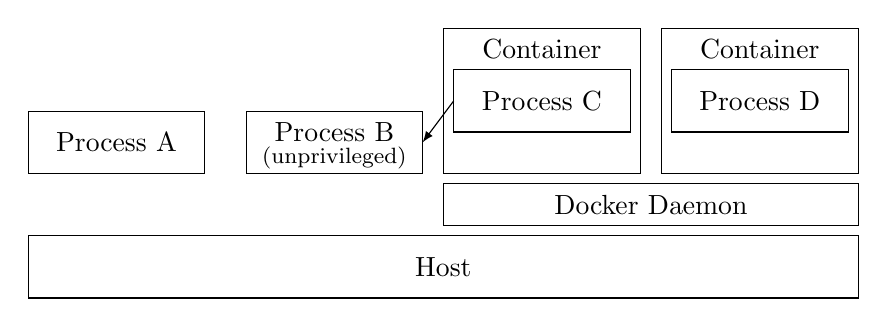
\begin{tikzpicture}[x=0.75pt,y=0.75pt,yscale=-1,xscale=1]
        % Host Rectangle
        \draw (0,100) -- (400,100) -- (400,130) -- (0,130) -- cycle ;
        \draw (200, 115) node {Host};

        %Docker Daemon Rectangle
        \draw (200,75) -- (400,75) -- (400,95) -- (200,95) -- cycle ;
        \draw (300,85) node {Docker Daemon};

        % Process A Rectangle
        \draw (0,40) -- (85,40) -- (85,70) -- (0,70) -- cycle ;
        \draw (42.5,55) node {Process A};

        % Process B Rectangle
        \draw (105,40) -- (190,40) -- (190,70) -- (105,70) -- cycle ;
        \draw (147.5,50) node {Process B};
        \draw (147.5,62.5) node {{\footnotesize (unprivileged)}};

        %Container Process C Rectangle
        \draw (200,0) -- (295,0) -- (295,70) -- (200,70) -- cycle ;
        \draw (247.5,10) node {Container};

        %% Process C Rectangle
        \draw (205,20) -- (290,20) -- (290,50) -- (205,50) -- cycle ;
        \draw (247.5,35) node {Process C};

        %Container Process D Rectangle
        \draw (305,0) -- (400,0) -- (400,70) -- (305,70) -- cycle ;
        \draw (352.5,10) node {Container};

        %% Process D Rectangle
        \draw (310,20) -- (395,20) -- (395,50) -- (310,50) -- cycle ;
        \draw (352.5,35) node {Process D};

        % Line
        \draw [latex-] (190,55) -- (205,35) ;
    \end{tikzpicture}
    \caption{}\label{fig:container-escape}
    \medskip
    \small
    A process (Process C) running inside a container accessing data on the host (that it should not be able to access), in this case Process B.
\end{figure}

\hfill

An example attack scenario would be a company that offers a PaaS (Platform as a Service) products that allows customers to run dockers on their infrastructure\footnote{This is actually quite common nowadays. All major computing providers offer such a service.}. If it is possible for the attacker to submit a Docker image that escapes the container and access the underlying infrastructure, they could access other containers or even other internal resources. That would, obviously, be a very big problem for that company.

\hfill

A lot of the known container escapes are possible because the container can access some files on the host. For example, if Docker mounts some necessary directories in \lstinline{/proc} by default (which would be a vulnerability) or if sensitive data is mounted as a volume (which would be a misconfiguration).

\hfill

As noted before, because a container uses the same kernel and resources as the host, an exploit granting root can be just as devastating run inside as outside of the docker, because the target kernel and resources are the same. CVE--2016--5195(Dirty Cow)\footnote{\url{https://dirtycow.ninja/}} is a good example of an exploit that allows container escapes\cite{Dirty-Cow-Escape}.

It should also be noted that an exploit that allows someone to escape from a Linux \lstinline{namespace} is essentially a container escape exploit. CVE--2017--7308\cite{CVE-2017-7308} is a good example of this.
